% $Header: /cvsroot/latex-beamer/latex-beamer/solutions/conference-talks/conference-ornate-20min.en.tex,v 1.6 2004/10/07 20:53:08 tantau Exp $

\documentclass{beamer}
%\documentclass[handout]{beamer}
%\usepackage{pgfpages}
%\pgfpagesuselayout{2 on 1}[a4paper,border shrink=5mm]

% This file is a solution template for:

% - Talk at a conference/colloquium.
% - Talk length is about 20min.
% - Style is ornate.



% Copyright 2004 by Till Tantau <tantau@users.sourceforge.net>.
%
% In principle, this file can be redistributed and/or modified under
% the terms of the GNU Public License, version 2.
%
% However, this file is supposed to be a template to be modified
% for your own needs. For this reason, if you use this file as a
% template and not specifically distribute it as part of a another
% package/program, I grant the extra permission to freely copy and
% modify this file as you see fit and even to delete this copyright
% notice.


\mode<presentation>
{
%  \usetheme{Warsaw}
%  \usetheme{Boadilla}
%  \usetheme{Goettingen}
%  \usetheme{Hannover}
%  \usetheme{Madrid}
%  \usetheme{Marburg}
%  \usetheme{Montpellier}
%  \usetheme{Pittsburgh}
  \usetheme{Hawke}
  % or ...

  \setbeamercovered{transparent}
  % or whatever (possibly just delete it)
}


\usepackage[english]{babel}
% or whatever

\usepackage[latin1]{inputenc}
% or whatever

\usepackage{times}
\usepackage[T1]{fontenc}
% Or whatever. Note that the encoding and the font should match. If T1
% does not look nice, try deleting the line with the fontenc.

\usepackage{multimedia}


%%%%%%
% My Commands
%%%%%%

\newcommand{\ml}{{\sc matlab}}
\newcommand{\bb}{{\boldsymbol{b}}}
\newcommand{\bx}{{\boldsymbol{x}}}
\newcommand{\by}{{\boldsymbol{y}}}
\newcommand{\bfm}[1]{{\boldsymbol{#1}}}

%%%%

\title[Lecture 14] % (optional, use only with long paper titles)
{Lecture 14 - Initial Value Problems}

% \subtitle
% {Include Only If Paper Has a Subtitle}

\author[I. Hawke] % (optional, use only with lots of authors)
{I.~Hawke}
% - Give the names in the same order as the appear in the paper.
% - Use the \inst{?} command only if the authors have different
%   affiliation.

\institute[University of Southampton] % (optional, but mostly needed)
{
%  \inst{1}%
  School of Mathematics, \\
  University of Southampton, UK
}
% - Use the \inst command only if there are several affiliations.
% - Keep it simple, no one is interested in your street address.

\date[Semester 1] % (optional, should be abbreviation of conference name)
{MATH3018/6141, Semester 1}
% - Either use conference name or its abbreviation.
% - Not really informative to the audience, more for people (including
%   yourself) who are reading the slides online

\subject{Numerical methods}
% This is only inserted into the PDF information catalog. Can be left
% out.



% If you have a file called "university-logo-filename.xxx", where xxx
% is a graphic format that can be processed by latex or pdflatex,
% resp., then you can add a logo as follows:

\pgfdeclareimage[height=0.5cm]{university-logo}{mathematics_7469}
\logo{\pgfuseimage{university-logo}}



% Delete this, if you do not want the table of contents to pop up at
% the beginning of each subsection:
%  \AtBeginSubsection[]
%  {
%    \begin{frame}<beamer>
%      \frametitle{Outline}
%      \tableofcontents[currentsection,currentsubsection]
%    \end{frame}
%  }
\AtBeginSection[]
{
  \begin{frame}<beamer>
    \frametitle{Outline}
    \tableofcontents[currentsection]
  \end{frame}
}


% If you wish to uncover everything in a step-wise fashion, uncomment
% the following command:

%\beamerdefaultoverlayspecification{<+->}


\begin{document}

\begin{frame}
  \titlepage
\end{frame}

\section{Ordinary Differential Equations}

\subsection{Ordinary Differential Equations}

\begin{frame}
  \frametitle{Ordinary Differential Equations}

  Consider first order systems of ordinary differential
  equations (ODEs), written
  \begin{equation*}
    \by'(x) = \bfm{f}(x, \by(x)).
  \end{equation*}
  Solution: any function $\by(x)$ that satisfies the equation. \pause

  \vspace{1ex}

  There are many possible solutions; for a \emph{unique} solution need
  to specify $n$ independent conditions (for system size $n$). \pause

  \vspace{1ex}

  When the $n$ conditions all specified at one point, e.g.
  \begin{equation*}
    \by(0) = \by_0,
  \end{equation*}
  this is an \emph{initial value problem}.

\end{frame}

\begin{frame}
  \frametitle{Getting to the first order form}

  The ODE need not be written in first order form, e.g.\
  \begin{equation*}
    z'' + z' + 1 = 0, \quad z(0) = a, \,\, z'(0) = b.
  \end{equation*} \pause

  Can recast the problem using \emph{auxilliary variables}, such as $w
  = z'$. \pause Result:
  \begin{equation*}
    \begin{pmatrix}
      w \\ z
    \end{pmatrix}' =
    \begin{pmatrix}
      -w - 1 \\ w
    \end{pmatrix}, \quad z(0) = a, \, \, w(0) = b.
  \end{equation*} \pause

  It is not always best to use simple derivatives as auxilliary
  variables. Example:
  \begin{equation*}
    \tfrac{1}{r^2} \left( r^2 P' / \rho \right)' = - 4 \pi \rho.
  \end{equation*}
  Use $P(r)$ and auxilliary variable
  \begin{equation*}
    \Pi(r) = r^2 P' / \rho.
  \end{equation*}

\end{frame}


\subsection{Numerical differentiation}

\begin{frame}
  \frametitle{Numerical differentiation}

  Assume value of $f(x)$ known at points $\{ x_j \}$. One approach
  uses these values to compute the derivative. \pause Simple example:
  assume $f(x)$ is known at $x_0$ and $x_0 \pm h$ for some small step
  $h$. \pause

  \vspace{1ex}

  Fit a linear polynomial $g$ (a straight line) to the values of $f(x)$ at
  $\{x_0, x_0 + h\}$: the derivative in this interval is the slope of
  the line
  \begin{equation*}
    f'(x_0) \simeq g'(x_0) = \frac{f(x_0 + h) - f(x_0)}{h}.
  \end{equation*}
  This is the \emph{forward difference} estimate of the derivative.
  \pause

  \vspace{1ex}

  Similarly, a linear fit in $[x_0 - h, x_0]$ gives
  \begin{equation*}
    f'(x_0) \simeq g'(x_0)  = \frac{f(x_0) - f(x_0 - h)}{h}.
  \end{equation*}
  This is the \emph{backward difference} estimate of the derivative.

\end{frame}

\begin{frame}
  \frametitle{Numerical differentiation - accuracy}

  \begin{equation*}
    f'(x_0) \simeq g'(x_0) = \frac{f(x_0 + h) - f(x_0)}{h}.
  \end{equation*}
  The accuracy of the approximation depends on the choice of
  interpolating polynomial. \pause

  \vspace{1ex}

  Check accuracy using Taylor expansion:
  \begin{align*}
    && f(x_0 + h) & = f(x_0) + h f'(x_0) + \tfrac{h^2}{2!} f''(x_0) +
    {\cal O}(h^3) \\
    \Rightarrow && \frac{f(x_0 + h) - f(x_0)}{h} & = \frac{f(x_0) + h
      f'(x_0) + \tfrac{h^2}{2!} f''(x_0) + {\cal O}(h^3) - f(x_0)}{h}
    \\
    &&& = f'(x_0) + {\cal O}(h).
  \end{align*} \pause

  \vspace{1ex}

  The same accuracy result holds for
  \begin{equation*}
    f'(x_0) = \frac{f(x_0) - f(x_0 - h)}{h}.
  \end{equation*}

\end{frame}

\begin{frame}
  \frametitle{Example}

  Compute the derivative of $f(x) = e^{x}$ at $x=0$ using forward
  differencing,
  \begin{equation*}
    f'(x_0) = \frac{f(x_0 + h) - f(x_0)}{h},
  \end{equation*}
  checking the error to the exact result $f'(0) \equiv 1$.
  \begin{center}
    \begin{tabular}{c|c c c c}
      $h$ & Formula & $f'_h(0)$ & $e_h$ & Error ratio \\[0.5ex] \hline
      0.5 & \rule{0pt}{1.5em} $\frac{\exp(0.5) - \exp(0)}{0.5}$ & 1.297 & 0.297 & -- \\
      0.05 & \rule{0pt}{1.5em} $\frac{\exp(0.05) - \exp(0)}{0.05}$ & 1.0254 & 0.0254 &
      0.085 \\
      0.005 & \rule{0pt}{1.5em} $\frac{\exp(0.005) - \exp(0)}{0.005}$ & 1.00250 & 0.0025 &
      0.098
    \end{tabular}
  \end{center}

  \vspace{1ex}

  The error ratio is (asymptotically) the same as the step-size ratio.

\end{frame}

\begin{frame}
  \frametitle{Central differencing}

  For more accuracy use a quadratic through the points $\{x_0 - h,
  x_0, x_0 + h\}$:
  \begin{equation*}
    f(x) \simeq g(x) = \alpha (x - x_0)^2 + \beta (x - x_0) + \gamma.
  \end{equation*}
  Compute the derivative at $x_0$:
  \begin{equation*}
    f'(x_0) = \beta = \frac{f(x_0 + h) - f(x_0 - h)}{2 h}.
  \end{equation*} \pause

  \vspace{1ex}

  This \emph{central differencing} estimate is more accurate than
  forward/backward differencing:
  \begin{equation*}
    \frac{f(x_0 + h) - f(x_0 - h)}{2 h} = f'(x_0) + {\cal O}(h^2).
  \end{equation*}

\end{frame}

\begin{frame}
  \frametitle{Example}

  Compute the derivative of $f(x) = e^{x}$ at $x=0$ with central
  differencing,
  \begin{equation*}
    f'(x_0) = \frac{f(x_0 + h) - f(x_0 - h)}{2 h},
  \end{equation*}
  checking the error to the exact result $f'(0) \equiv 1$.
  \begin{center}
    \begin{tabular}{c|c c c}
      $h$ & Formula & $f'_h(0)$  & Error ratio \\ \hline
      0.5 & \rule{0pt}{1.5em} $\frac{\exp(0.5) - \exp(-0.5)}{1}$ & 1.042  & -- \\
      0.05 & \rule{0pt}{1.5em} $\frac{\exp(0.05) - \exp(-0.05)}{0.1}$ & 1.0004167 &
      0.00988 \\
      0.005 & \rule{0pt}{1.5em} $\frac{\exp(0.005) - \exp(-0.005)}{0.01}$ & 1.0000004180
      & 0.0100
    \end{tabular}
  \end{center}
  Central differencing is much more accurate, and the error ratio is
  (asymptotically) the \emph{square} of the step-size ratio.

\end{frame}

\begin{frame}
  \frametitle{Other numerical differencing formulas}

  \begin{itemize}
  \item Intuitively, use of information from both sides of $x_0$ leads
    to higher accuracy (e.g.\ central differencing). \pause
  \item Can build differencing formulas directly from Taylor
    series. No interpolating function, but are equally valid.  \pause
  \item Estimates of higher derivatives can use interpolation approach
    or repeated numerical differencing. For example, estimate $f''(x)$
    using forward and backward differencing:
    \begin{align*}
      f''(x_0) & \simeq \frac{f'(x_0) - f'(x_0 - h)}{h} \\
               & \simeq \frac{\left(f(x_0 + h) - f(x_0) \right) -
                 \left(f(x_0) - f(x_0 - h) \right)}{h^2} \\
               & = \frac{f(x_0 + h) + f(x_0 - h) - 2 f(x_0)}{h^2}.
    \end{align*}
  \end{itemize}
\end{frame}


\subsection{Euler's method}


\begin{frame}
  \frametitle{Euler's method}

  Using differencing construct the simplest method for solving
  \begin{equation*}
    \by'(x) = \bfm{f}(x, \by(x)), \quad \by(0) = \by_0.
  \end{equation*}
  Using step size $h$, apply forward differencing to $\by$:
  \begin{equation*}
    \frac{\by_{n+1} - \by_n}{h} = \bfm{f}(x_n, \by_n) \quad
    \Rightarrow \quad \by_{n+1}  = \by_n + h \bfm{f}(x_n, \by_n).
  \end{equation*} \pause
  Given initial data $\by_0$, for each stage we can compute
  $\by_{n+1}$ from data $\by_n$. Methods of this sort are called
  \emph{explicit}. \pause

  \vspace{1ex}

  Compute the error using Taylor expansion:
  \begin{equation*}
    \by_{n+1} \equiv \by \left(x_0 + (n+1) h \right) = \by_n + h
    \bfm{f}(x_n, \by_n) + {\cal O}(h^2).
  \end{equation*} \pause
  This means the \emph{local} error is ${\cal O}(h^2)$, not the global
  error.

\end{frame}

\begin{frame}
  \frametitle{Example}

  Apply Euler's method to
  \begin{equation*}
    y'(x) = - \sin(x), \quad y(0) = 1
  \end{equation*}
  up to $x = 0.5$. Using step size $h = 0.1$ gives
  \begin{center}
    \begin{tabular}{c|c c c c}
      $n$ & $x_n$ & $y_n$ & $f(x_n, y_n) = -\sin(x_n)$ & $\cos(x_n)$ \\
      \hline
      0 & 0.0 & 1.00  &  0.000 & 1.000 \\
      1 & 0.1 & 1.00  & -0.100 & 0.995 \\
      2 & 0.2 & 0.99  & -0.199 & 0.980 \\
      3 & 0.3 & 0.97  & -0.296 & 0.955 \\
      4 & 0.4 & 0.94  & -0.389 & 0.921 \\
      5 & 0.5 & 0.90  &        & 0.878
    \end{tabular}
  \end{center} \pause
  The error is $2.4\%$; using $h = 0.01$ the final result is $y_{50} =
  0.880$, an error of $0.24\%$: first order convergence.

\end{frame}

\begin{frame}
  \frametitle{Convergence}

  \begin{center}
    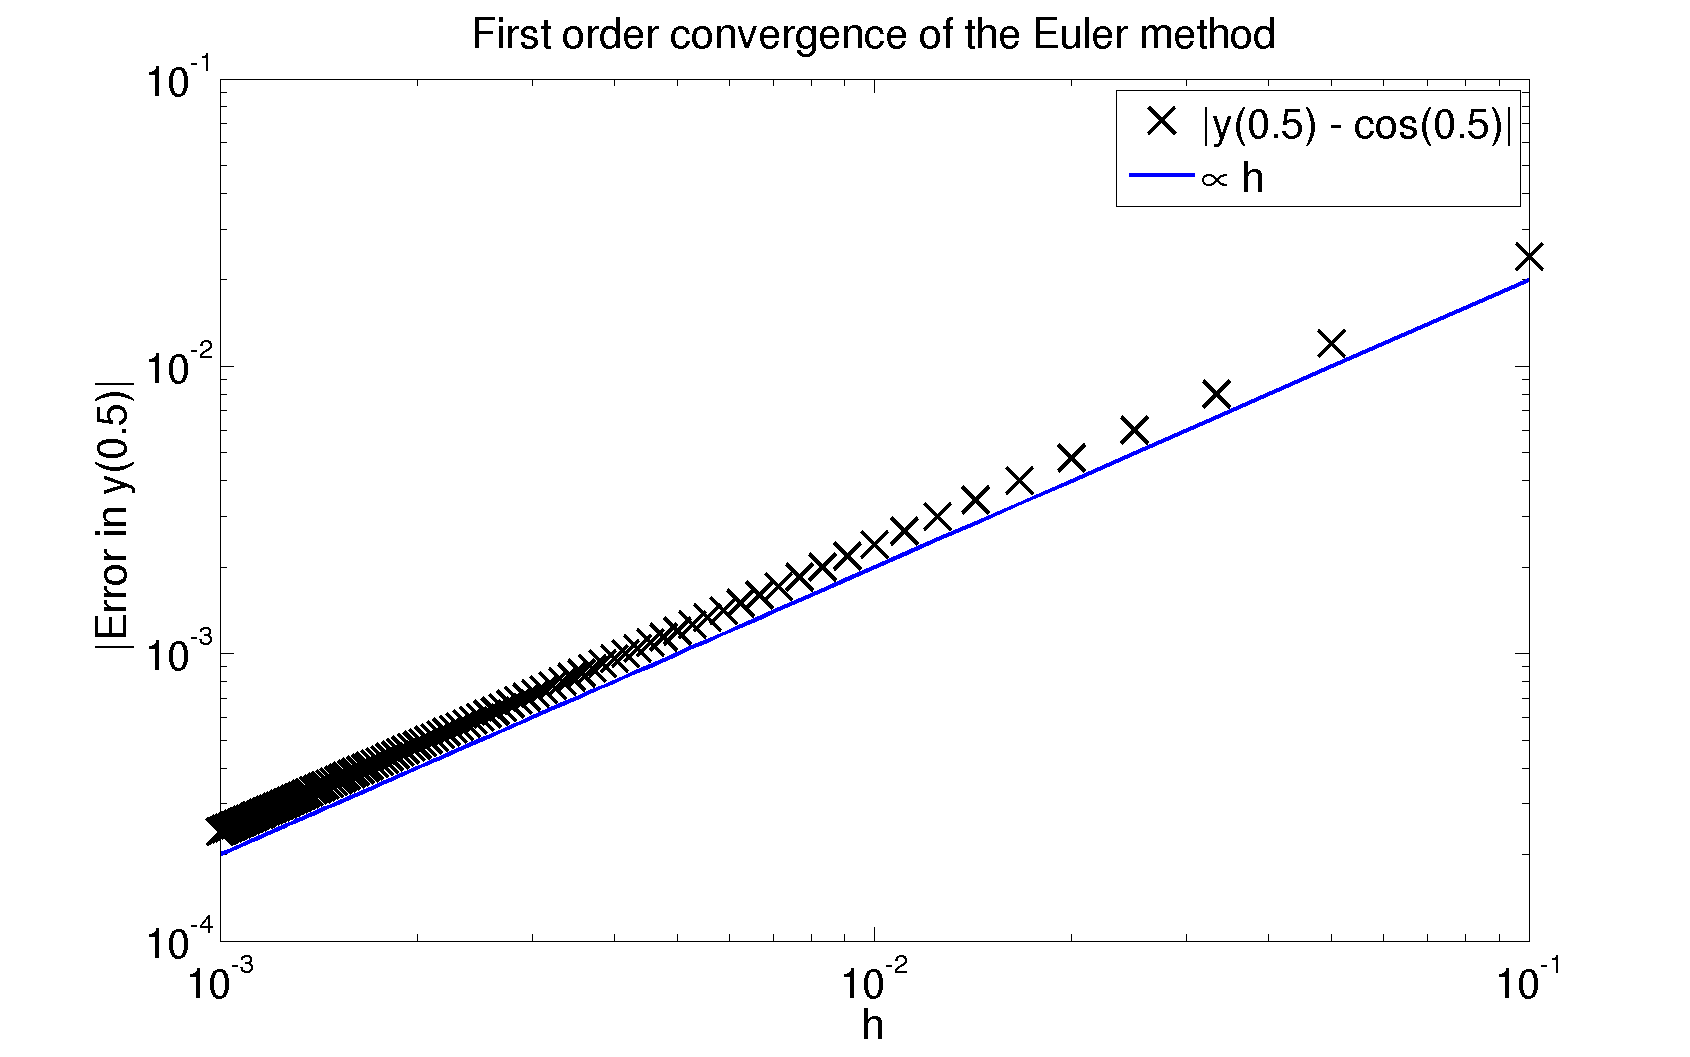
\includegraphics[height=0.7\textheight]{figures/EulerSinConvergence}
  \end{center}
   More conclusive evidence that the convergence of Euler's method is
   first order: the global error is $\propto h$.

\end{frame}

\begin{frame}
  \frametitle{Example: 2}


  Consider the system
  \begin{equation*}
    \left\{
      \begin{aligned}
        \dot{x} & = -y \\ \dot{y} & = x
      \end{aligned} \right., \quad x(0) = 1, \, \, y(0) = 0.
  \end{equation*}
  In polar coordinates this is $\dot{r} = 0$, $\dot{\phi} = 1$.
  \begin{columns}
    \begin{column}{0.5\textwidth}
      \begin{overlayarea}{\textwidth}{0.4\textheight}
        \only<2-3|handout:1>
        {
          Use Euler's method with $h=0.1$. At $t=50$ the result is
          slightly out of phase and the radius has grown
          significantly.

        }
        \only<3|handout:1>
        {
          \vspace{1ex}

          With $h = 0.01$ the errors are smaller, but still visible.
        }
      \end{overlayarea}
    \end{column}
    \begin{column}{0.5\textwidth}
      \begin{overlayarea}{\textwidth}{0.6\textheight}
        \only<2|handout:0>
        {
          \begin{center}
            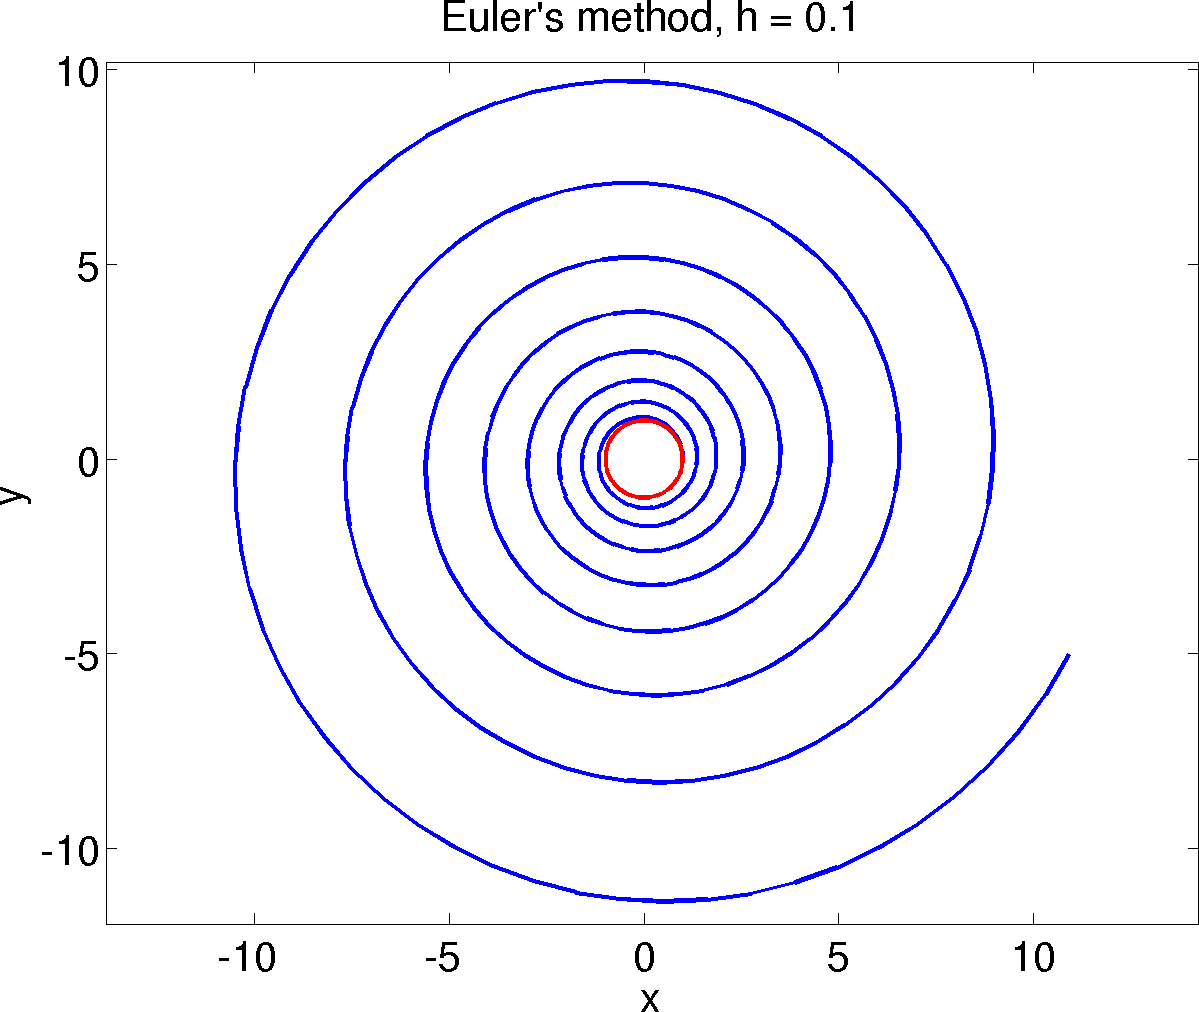
\includegraphics[height=0.5\textheight]{figures/EulerPlot1_crop}
          \end{center}
        }
        \only<3|handout:1>
        {
          \begin{center}
            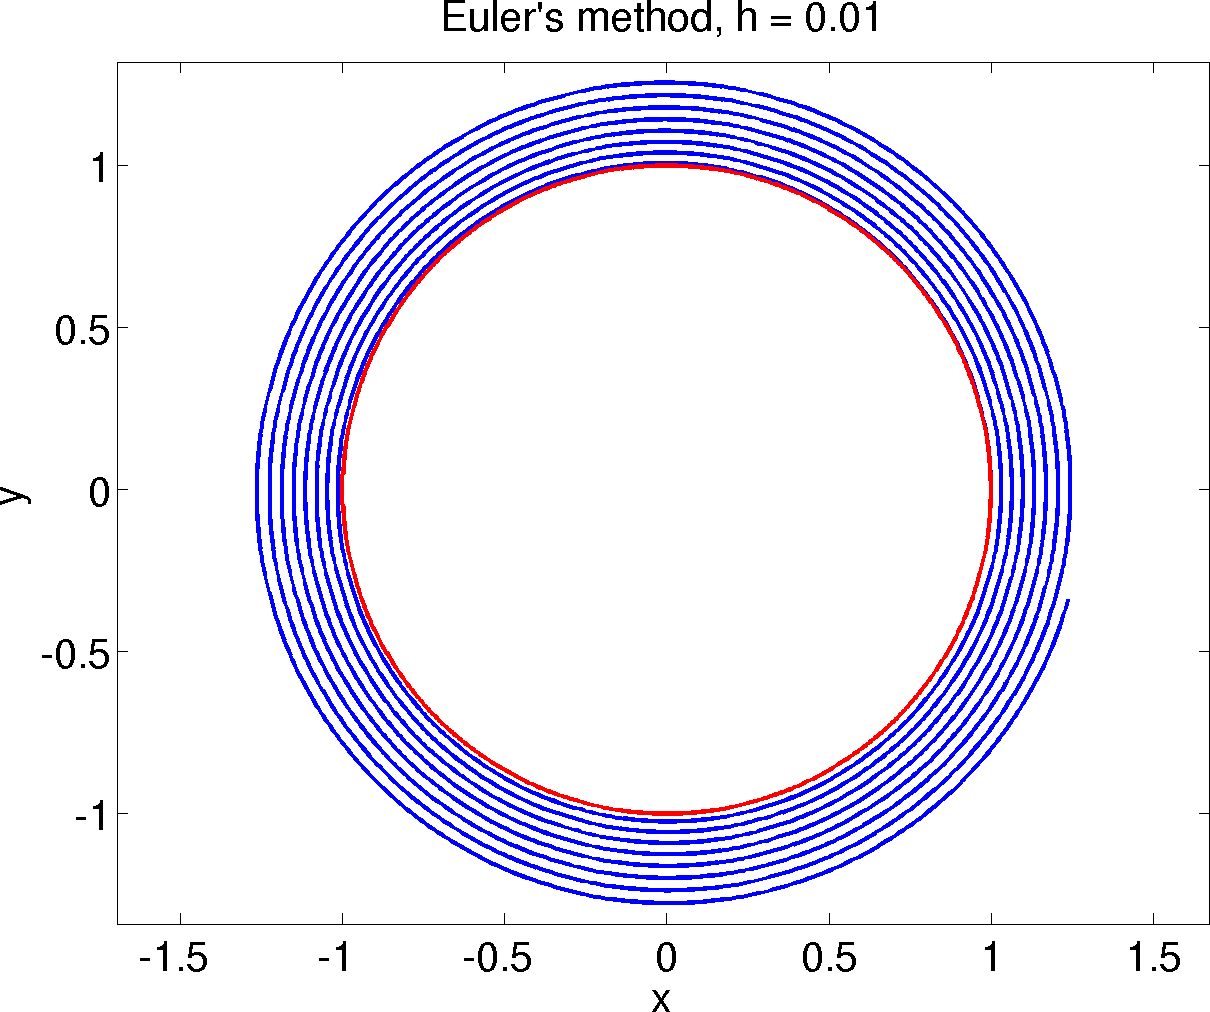
\includegraphics[height=0.5\textheight]{figures/EulerPlot2_crop}
          \end{center}
        }
      \end{overlayarea}
    \end{column}
  \end{columns}

\end{frame}

\begin{frame}
  \frametitle{Convergence: 2}

  \begin{center}
    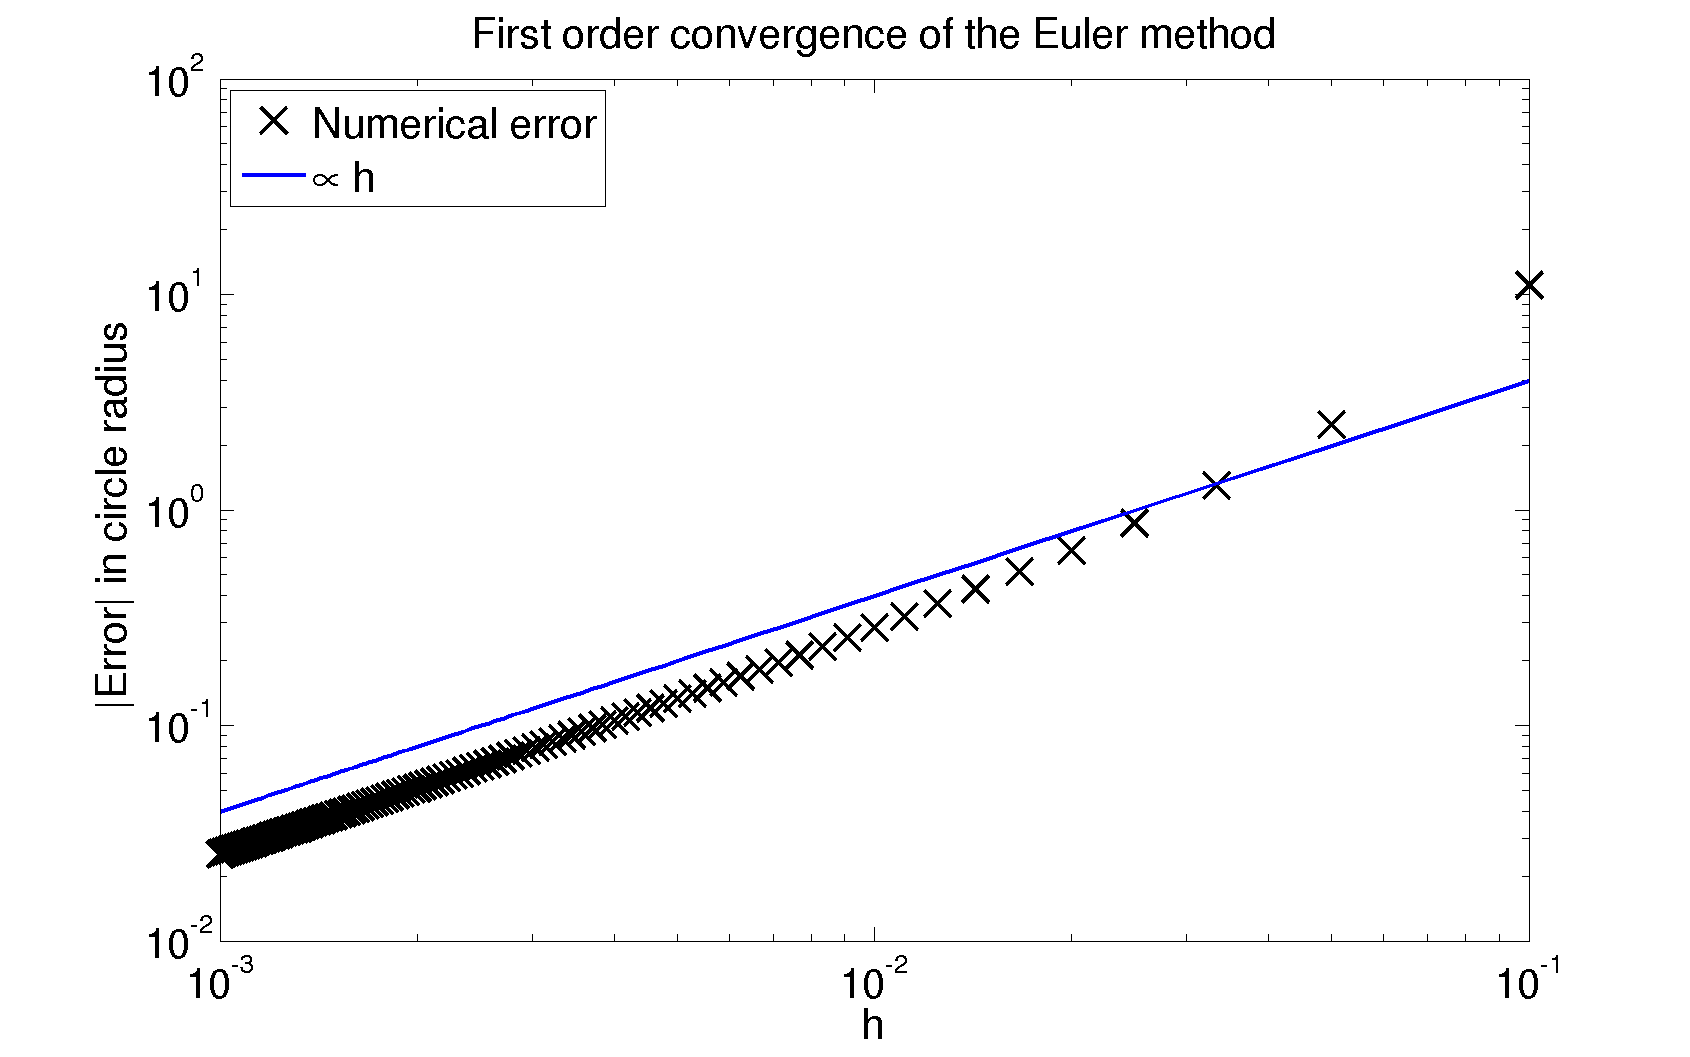
\includegraphics[height=0.7\textheight]{figures/EulerCircleConvergence}
  \end{center}
  More conclusive evidence that the convergence of Euler's method is
  (asymptotically) first order: the global error is $\propto h$.

\end{frame}


\section{Summary}

\subsection{Summary}

\begin{frame}
  \frametitle{Summary}

  \begin{itemize}
  \item Initial value problems are ODEs specified by an initial
    condition $\by(0) = \by_0$.
  \item Numerical differentiation using finite differences can easily produce
    \begin{itemize}
    \item first order accurate approximations to $f'(x)$ using
      \emph{forward} or \emph{backward} differencing, or
    \item second order accurate approximations to $f'(x)$ using
      central differencing.
    \end{itemize}
  \item General central differencing about $x_i$ uses the closest
    points to $x_i$ in a symmetric fashion to approximate whichever
    derivative is required.
  \item To prove the convergence behaviour Taylor's theorem is used.
  \item Approximations to higher derivatives are also easy to compute.
  \item Using forward differencing in the IVP gives Euler's method.
  \item Euler's method has a local error $\propto h^2$, and a global
    error $\propto h$.
  \end{itemize}

\end{frame}

\end{document}



%%% Local Variables:
%%% mode: latex
%%% TeX-master: t
%%% End:
